
\section{Background and Situation}

In many industries, people are required to collect and structure information in standardized formats such as forms, logs, or reports. This process, known as \textit{template filling}, is employed in various industries, including healthcare~\cite{du2021template}, manufacturing~\cite{wang2021spoken}, web-based automation~\cite{chen2024webform}, and customer service platforms~\cite{sun2023slot}. In these environments, structured data entry is crucial for ensuring operational continuity, regulatory compliance, and decision-making. For instance, hospital staff must document symptoms and treatments using structured intake forms, while factory operators fill out reports on equipment performance, safety incidents, and shift summaries.

Traditionally, template filling has been performed manually, either by writing on paper or typing into digital forms. However, these methods can be time-consuming, error-prone, and impractical in settings where hands-free operation is needed or workers are under time pressure. For example, a field technician wearing protective gear may not have the ability to type during operations. In such cases, \textit{speech-based template filling} offers a promising alternative by allowing users to dictate their inputs instead of entering them by hand~\cite{wang2021spoken}.

This shift toward voice interaction is made possible by recent progress in artificial intelligence, particularly in \textit{automatic speech recognition (ASR)} and \textit{large language models (LLMs)}. ASR systems like OpenAI’s Whisper have achieved strong performance in transcribing speech accurately, even in noisy or informal conditions~\cite{radford2023whisper, fathullah2023prompting}. These models can handle multiple accents, technical terminology, and varying background noise, making them suitable for real-world applications such as hospitals and factories~\cite{wang2021spoken}.

Meanwhile, LLMs such as GPT-4 and Claude have transformed natural language processing by enabling machines to understand context, extract relevant information, and generate structured outputs from unstructured inputs~\cite{du2021template, schick2023toolformer}. These models are capable of filling out complex templates if given the correct input format, and can even infer missing details or resolve ambiguities in the user's statements~\cite{mialon2023augmented}.

However, current systems that combine ASR and LLMs often use a \textit{monolithic architecture}, where a single model performs the entire task of understanding and filling out the form~\cite{sun2023slot, chen2024webform}. While this approach is simple to implement, it lacks flexibility and interpretability. Errors are hard to trace back to a specific step, and adapting the system to a new form or domain usually requires retraining the entire pipeline~\cite{liu2022conversational, schick2023toolformer}. This becomes especially problematic when dealing with spoken inputs, which can be disfluent, unordered, or incomplete~\cite{fathullah2023prompting}.

As a response to these limitations, recent research suggests using \textit{modular or multi-agent architectures}, where each component of the system (e.g., transcription, field identification, value extraction) is handled separately~\cite{mialon2023augmented, schick2023toolformer}. This design enables better control, easier debugging, and smoother integration of new improvements. This thesis builds upon this idea by developing a modular system—called \textbf{Invox}—that focuses on speech-based template filling in realistic, industrial environments.


\section{Problem Description}

While recent advances in large language models (LLMs) and automatic speech recognition (ASR) have made it easier to build systems for filling out forms automatically, most existing solutions rely on a \textit{monolithic design}, where a single model handles the entire task of understanding input and generating all required field values in one step. For instance, Du et al.~\cite{du2021template} propose zero-shot prompting to generate complete templates from unstructured text, while Sun et al.~\cite{sun2023slot} introduce a slot-filling pipeline for spoken input that decodes all fields in a unified pass. Similarly, Chen et al.~\cite{chen2024webform} apply large language models to populate web-based forms via single-shot prompts. Although effective in controlled settings, such monolithic approaches become brittle when processing real-world spoken input, which is often disfluent, incomplete, noisy, or non-linear—making these systems hard to adapt, debug, or extend across domains.


One major issue is \textit{fragility}. These models are often trained on specific types of inputs or formats, and they may fail when the input varies slightly—such as when someone uses uncommon phrasing, mixes up the order of fields, or leaves out certain information~\cite{fathullah2023prompting, liu2022conversational}. This is common in real-world situations, where people speak naturally and often provide extra details, use abbreviations, or skip fields they assume are obvious. When a monolithic model encounters this variation, it might leave fields blank, insert wrong values, or produce inconsistent results~\cite{wang2021spoken, sun2023slot}.

Another major challenge is \textit{lack of transparency}. When a single model does the entire job, it is difficult to figure out what went wrong if the result is incorrect. For example, was the problem caused by a transcription error, misunderstanding of the content, or a failure in mapping the answer to the correct field? Because all steps are handled together, it is hard to trace and fix errors, which limits the system’s reliability and maintainability~\cite{schick2023toolformer}.

Additionally, current systems are \textit{hard to customize} for different industries or forms. Each form may have its own structure, required fields, and domain-specific language. Changing the model to handle a new type of report or form often means retraining or redesigning the entire system~\cite{du2021template, mialon2023augmented}. This makes it expensive and time-consuming to adapt these systems to new domains.

These problems are even more pronounced when the input comes from \textit{spoken language}, where transcription errors, filler words, background noise, and informal speaking patterns make the task even harder~\cite{radford2023whisper, fathullah2023prompting}. As a result, current one-step systems often fail in real-world use cases where the input is imperfect, the domain is specialized, or the system needs to adapt over time.

To solve these problems, there is a need for a more flexible, transparent, and modular approach that separates the process into smaller, understandable steps. This allows better error handling, easier debugging, and faster adaptation to new use cases~\cite{mialon2023augmented, schick2023toolformer}.

\section{Motivating Scenario}

To illustrate the challenges of template filling in real-world environments, consider a typical shift in the \textit{steel manufacturing industry}.

Steel plant operators work under intense conditions—loud machinery, high heat, and strict production deadlines. At the end of each 8-hour shift, they are expected to submit a \textit{shift report} documenting safety incidents, equipment issues, production figures, and handover notes. These reports are essential for maintaining operational continuity, safety compliance, and accountability. Yet in practice, workers often fill them out hastily—sometimes incompletely or not at all—especially during late-night shifts or when fatigued.

To reduce effort, many workers have turned to voice-based reporting. They record verbal summaries using mobile phones or handheld devices, describing what happened during the shift in their own words. While this captures richer context, the burden then shifts to someone else—often a supervisor—who must listen to the recordings and manually transcribe relevant details into structured forms.

Now imagine an intelligent system that could take these raw audio notes, transcribe them, interpret their meaning, and fill in the shift report automatically. For instance, if a worker says:

\begin{quote}
``We had a minor safety incident near the blast furnace around 2 p.m.—someone tripped, but no injuries. Conveyor belt on Line B stopped twice, restarted after 10 minutes each time. Production target met—482 tons.''
\end{quote}

Such a system would ideally extract structured information like:
\begin{itemize}
    \item \textbf{Safety Incident:} Minor, near blast furnace, no injuries
    \item \textbf{Time:} Around 2 p.m.
    \item \textbf{Equipment Issue:} Line B conveyor belt stopped twice
    \item \textbf{Production:} 482 tons
\end{itemize}

\begin{figure}[ht]
    \centering
    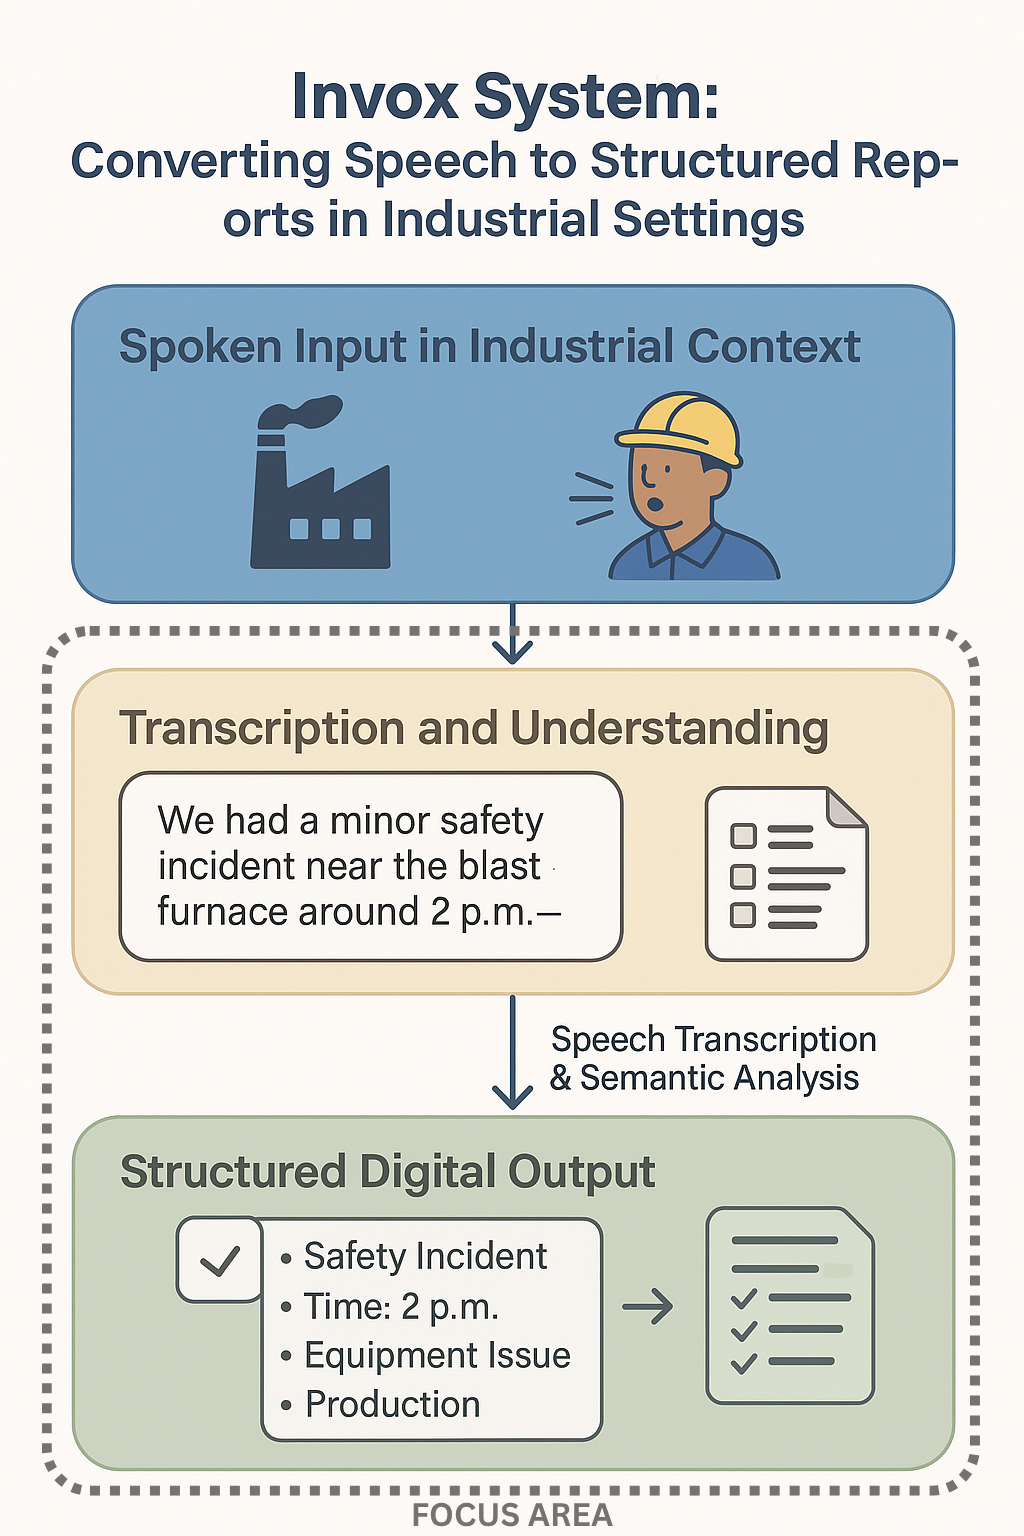
\includegraphics[scale=0.35]{images/Motivation.png}
    \caption{Invox: From spoken input to structured report}
    \label{fig:invox-motivation}
\end{figure}

Although this task may seem straightforward, it is far from trivial. Spoken input is often informal, unordered, and filled with vague expressions or filler words. Terms like “blast furnace” or “Line B” reflect domain-specific knowledge that the system must understand. Noise, fatigue, and rushed speech introduce further variability.

This scenario reveals four core challenges:
\begin{itemize}
    \item \textbf{Unstructured input:} Workers speak naturally, not in pre-defined templates.
    \item \textbf{Domain-specific language:} Technical terms and abbreviations must be recognized and interpreted.
    \item \textbf{Variability and noise:} Inconsistent phrasing, ambient noise, and disfluencies degrade transcription quality.
    \item \textbf{Template diversity:} Different departments use different reporting formats and vocabularies.
\end{itemize}

Together, these challenges underscore the need for a more intelligent and adaptable approach. A modular system like \textbf{Invox}, capable of processing speech, identifying relevant fields, and generating structured output, offers a scalable solution tailored to the complexities of real industrial environments.


\section{Scope of the Thesis}

This thesis is situated at the intersection of speech processing and natural language understanding, focusing on the task of converting noisy, unstructured spoken input into structured digital forms using large-scale pretrained models.

The primary use case addressed is shift documentation in the steel manufacturing industry. Operators in this domain often record verbal summaries at the end of their shifts, describing production events, safety incidents, and equipment issues. These recordings are typically informal, multilingual, and captured in noisy environments. This makes the use case ideal for evaluating robustness in low-structure, real-world input scenarios~\cite{wang2021spoken, fathullah2023prompting}.

The technical scope of this work includes the use of state-of-the-art automatic speech recognition (ASR) models—specifically OpenAI's Whisper~\cite{radford2023whisper}—combined with large language models (LLMs) such as GPT-5, Gemini-2.5-pro, etc. These components are orchestrated in a modular agent-based architecture for handling tasks like transcription interpretation, field-value mapping, and validation. No fine-tuning or training of models is performed; the focus is on system-level orchestration and domain-adapted prompt engineering.

The evaluation is limited to the accuracy and reliability of the structured output produced from recorded input. This thesis does not cover areas such as UI/UX design, live streaming input, conversational turn-taking, or the deployment of on-device inference. Instead, it aims to explore how existing ASR and LLM technologies can be effectively combined into a practical and scalable speech-based form filling system suitable for high-noise industrial domains.


\section{Objectives}

The main objective of this thesis is to design and evaluate a modular system—called \textbf{Invox}—that can automatically fill out structured forms using unstructured speech or text input. The system aims to overcome the limitations of current single-model, end-to-end solutions by introducing a flexible, multi-agent approach that separates the task into smaller, specialized components.

To achieve this goal, the following two specific objectives are defined:

\begin{enumerate}
    \item \textbf{Design a modular multi-agent architecture} for template filling that separates the process into subtasks such as transcription, field detection, answer generation, and verification—each handled by a dedicated agent. This design supports flexibility, transparency, and domain adaptability. As part of this design, five distinct prompting strategies are implemented using large language models (LLMs), ranging from single-pass full-input methods to iterative multi-model consensus approaches. These strategies are chosen to reflect different trade-offs in accuracy, latency, cost, and interpretability.

    \item \textbf{Evaluate the system performance} using a hybrid strategy that combines standardized benchmarking and real-world testing. For benchmarking, the official MUC-4 evaluation protocol \cite{chinchor1992muc4} is applied, using slot-level precision, recall, and F1-score to compare structured information extraction. Finally, results from all prompting strategies are compared to identify the most effective architectural approach under various real-world conditions.
\end{enumerate}

These objectives guide the development and validation of a system that is not only technically sound but also practical and scalable in industrial settings.


\section{Document Outline}

Following this introduction, the thesis begins with a discussion of related work in the field. This includes an overview of existing systems for template filling, particularly those that use speech input or large language models. The literature is analyzed to identify current limitations and to derive a clear set of requirements for building a better, more modular solution.

Next, the conceptual foundation of the proposed system is introduced. The structure of Invox is explained, along with four different design strategies that use large language models in distinct ways. These approaches are described in detail, along with the reasoning behind each one and a discussion of possible alternatives.

After outlining the concept, the implementation is described. This includes the software architecture, technology choices, and how each component—such as speech transcription, RAG, field extraction, and answer verification—was built. Attention is given to how modularity was achieved to support maintainability and reuse.

The following part of the thesis presents the working prototype. Screenshots, mockups, and usage examples are used to demonstrate how the system operates in practice. The user interface and interactions are shown, illustrating how speech input can be turned into a structured form with minimal effort.

Once the system is introduced and demonstrated, the evaluation section presents a detailed analysis of its performance. A benchmark dataset is used to test the system across four architectural approaches. The results are analyzed using metrics such as accuracy, latency, consistency, and computational cost.

The final part of the thesis summarizes the key findings, reflects on the strengths and limitations of the current implementation, and proposes ideas for future research and system improvements.
